\documentclass[14ppt]{article}
\usepackage[utf8]{inputenc}
\usepackage{amsmath}
\usepackage{amsfonts}
\usepackage{graphicx}
\usepackage[colorinlistoftodos]{todonotes}
\usepackage[Algoritm]{algorithm}
\usepackage[noend]{algpseudocode}
\usepackage{txfonts}
\usepackage{url}
\usepackage{hyperref}
\usepackage{geometry}
\usepackage{romana}
\begin{document}
\begin{titlepage}
    \begin{center}
    \Large
        Universitatea din Craiova\\
        Facultatea de Automatică, Calculatoare și Electronică\\
         
\includegraphics[width=0.2\textwidth]{ace.png}
        \vspace*{2cm}
            
        \Huge{\textbf{Selectarea aspersoarelor}\\}
        \vspace{0.3cm}
        \Large
        Proiectarea algoritmilor
            
        \vspace{1.5cm}
            
        \Large \textbf{Student}\\ Smarandache Alexandru
        \\\vspace{0.25cm}
        \Large{\textbf{Calculatoare Română}}\\
        \Large{Grupa 1.2B}\\
         \Large{\textbf{Anul I}}\\
        \vfill
    
        \vspace{0.8cm}
            
        \Large
        Mai 2020
    \end{center}
\end{titlepage}

\section{Enunțul problemei}
 Se consideră \emph{n} aspersoare instalate să ude o bandă orizontală de iarbă ce are \emph{L} metri lungime și \emph{l} metri lățime. Fiecare aspersor este centrat vertical pe banda de iarbă respectivă. Pentru fiecare aspersor se cunosc: i) poziția sa ca distanță față de capătul din stânga al liniei care străbate pe orizontală mijlocul fâșiei de iarbă și respectiv ii) raza sa de operare. Să se determine numărul minim de aspersoare care trebuie pornite pentru a uda întreaga bandă de iarbă. Implementați 2 algoritmi diferiți. 

 
 \section{Algoritmii propuși}
\subsection{Motivarea alegerii}
Din enunț, observăm că problema se poate scrie ca o problemă geometrică în spațiul bidimensional: \\ Se consideră un dreptunghi de dimensiune \emph{L} *  \emph{l} și \emph{n} puncte centrate vertical pe linia care străbate pe orizontală mijlocul dreptunghiului. Aceste puncte reprezintă centre ale unor cercuri. Sunt cunoscute lungimea și lățimea dreptunghiului, numărul de puncte, poziția acestora ca distanță față de capătul din stânga al liniei care străbate pe orizontală mijlocul dreptunghiului și raza fiecărui cerc. Să se determine numărul minim de cercuri, a căror reuniune să cuprindă întregul dreptunghi. \\
Înainte de a trece la rezolvarea problemei, vom încerca reducerea ei la spațiul unidimensional. \\
Reprezentăm dreptunghiul în coordonate carteziene, astfel, cele 4 vârfuri vor avea următoarele coordonate: ( \emph{0}, \emph{$\frac{l}{2}$} ), ( \emph{L} , \emph{$\frac{l}{2}$} ), ( \emph{L} , \emph{-$\frac{l}{2}$} ),  ( \emph{0}, \emph{-$\frac{l}{2}$} ). Ținând cont că punctele sunt centrate vertical pe linia care străbate orizontal mijlocul dreptunghiului, dar și de simetria cercului și cea a dreptunghiului, pentru a rezolva problema trebuie să aflăm numărul minim de semicercuri a căror reuniune cuprinde dreptunghiul situat deasupra axei \emph{$Ox$}, adică dreptunghiul de coordonate: (\emph{0}, \emph{$\frac{l}{2}$} ), (\emph{L} , \emph{$\frac{l}{2}$}), (\emph{L} , \emph{0}),  (\emph{0}, \emph{0}). Din datele problemei, se observă că de interes este doar porțiunea semicercului care intersectează segmentul format de punctele (\emph{0}, \emph{$\frac{l}{2}$}) și (\emph{L}, \emph{$\frac{l}{2}$}), adică porțiunea semicercului pentru care, în coordonate carteziene: $\emph{$\frac{l}{2}$} \leq y \implies y - \emph{$\frac{l}{2}$} = \emph{0} \iff y = \emph{$\frac{l}{2}$}.$ \\ 
Din ecuația cercului:  $R^2$ $=$ $x^2 + y^2$  \implies $x^2 = R^2 - y^2$ $\iff x = \pm \[ \sqrt{R^2 - y^2} $.\\
Modulul lui \emph{x} se obține și prin aplicarea teoremei lui Pitagora: ipotenuza este segmentul format de punctele $(C,0)$ și $(x,\frac{l}{2})$, cateta opusă este segmentul alcătuit de punctele $(C+x,\frac{l}{2})$ și  $(C+x,0)$, iar cateta alăturată segmentul compus din punctele $(C,0)$ și $(C+x,0)$. Soluția rezultată este $|x| = \sqrt{R^2 - (\frac{l}{2})^2}$. 
\begin{center}
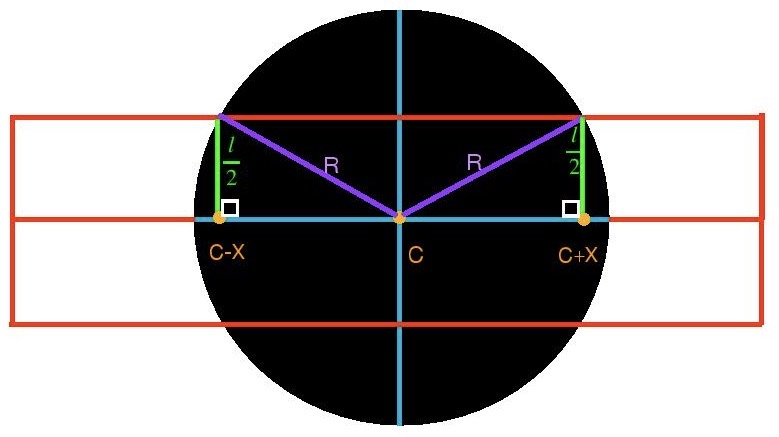
\includegraphics[ width = 9cm]{pitagora.jpeg}
\end{center}
Așadar, pentru x vom alege valoarea pozitivă, iar fiecare porțiune din cerc care ne interesează pentru dezvoltarea algoritmului devine un dreptunghi cu coordonatele: ($distanța - x$, \emph{0} ), ( \emph{distanța + x}, \emph{0} ), ( \emph{distanța - x}, \emph{$\frac{l}{2}$} ),   ( \emph{distanța + x}, \emph{$\frac{l}{2}$} ), unde distanța este depărtarea punctului de origine. De asemenea, dacă \emph{distanța - x} va fi mai mică decât 0, aceasta va primi valoarea 0, iar dacă \emph{distanța + x} va fi mai mare decât lungimea, aceasta va primi valoarea lungimii, pentru că de interes este doar porțiunea care face parte din dreptunghi.\\
În plan unidimensional, problema este similară cu: \\Se dau \emph{n} intervale de forma: $[a_1, b_1], ... ,[a_{n},{b_{n}]$ și un interval [\emph{0}, \emph{L}], unde: $ 0 \leq a_i \leq b_i \leq L, \forall i \in [\emph{1}, \emph{n}] $.  Intervalele au următoarea proprietate: $\forall x \in [\emph{0}, \emph{L}], x \in [a_1, b_1]\bigcup...\bigcup[a_{n},{b_{n}]$. Să se determine numărul minim de submulțimi disjuncte ale mulțimii de  $n$ intervale, astfel încât reuniunea intervalelor din fiecare submulțime să includă intervalul [\emph{0}, \emph{L}]. \\
\textbf{\emph{Observație: }} Sunt 3 cazuri particulare de intervale care nu sunt necesare pentru ca proprietatea să rămână adevărată, dacă vom completa intervalul $[0,L]$ de la stânga spre dreapta:
\begin{enumerate}
\item Fie $i_1, i_2 ... i_k \in [\emph{1}, \emph{n}]$, unde $i_1 \neq i_2 \neq ... \neq i_k$ și $1 \leq k \leq n$,  astfel încât $a_i_1 = a_i_2 = ... = a_i_k$ și $b_i_1 = b_i_2 = ... = b_i_k$, atunci $[a_i_2,b_i_2], ... , [a_i_k,b_i_k] $ nu sunt necesare. 
\item Fie $i_1, i_2 \in [\emph{1}, \emph{n}] $, unde: $ i_1 \neq i_2$ , astfel încât $a_i_1 \leq a_i_2$ și $b_i_2 < b_i_1$ sau $a_i_1 < a_i_2$ și $b_i_2 \leq b_i_1$, atunci $[a_i_2,b_i_2]$ nu este necesar.
\item Fie $i_1, i_2, i_3 \in [\emph{1}, \emph{n}], i_1 \neq i_2 \neq i_3$ , astfel încât $[a_i_2,b_i_2]$ $\subset$ ( $[a_i_1,b_i_1]\cup [a_i_3,b_i_3]$ ),unde $[a_i_1,b_i_1]$ este unul din intervale absolut necesare și $a_i_1 \leq a_i_2 \leq b_i_1$, $b_i_1 \leq b_i_2 \leq b_i_3$ și $a_i_3 \leq b_i_1$, atunci $[a_i_2,b_i_2]$ nu este necesar. 
\end{enumerate}
\begin{center}
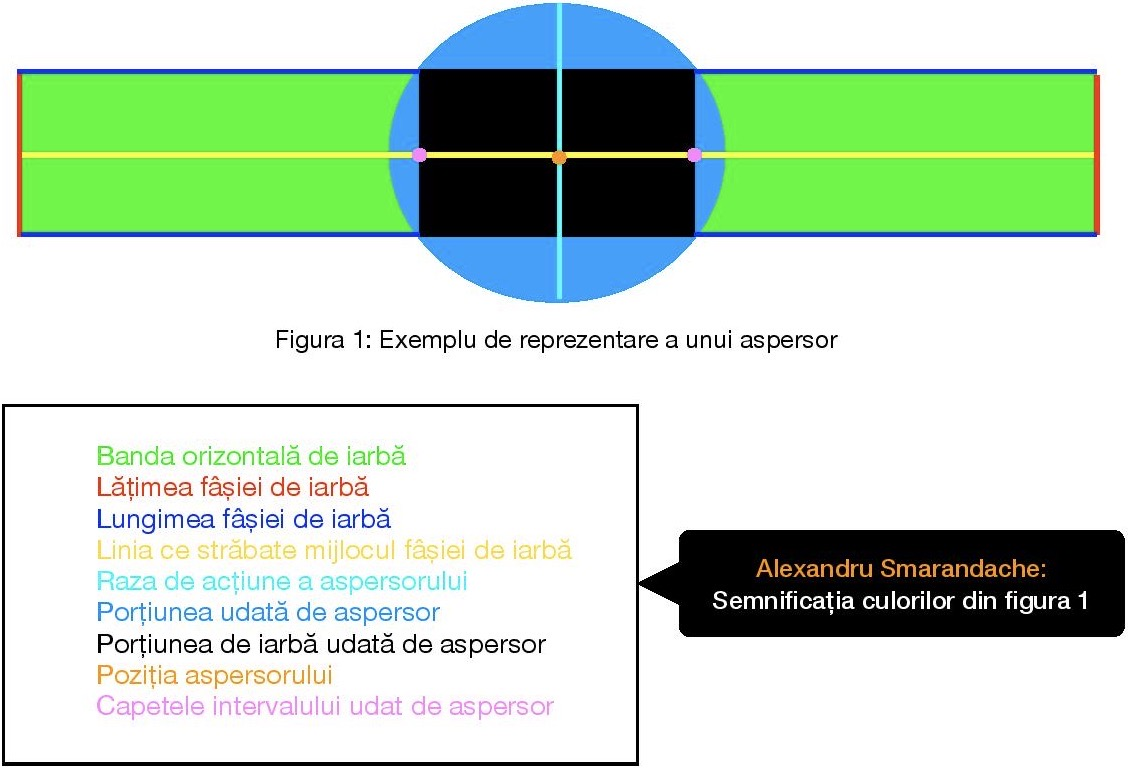
\includegraphics[ width = 15cm]{aspersor_gf-page-002.jpeg}
\end{center}

\subsection{Algoritmii}
\subsubsection{Primul algoritm propus}
\begin{enumerate}
 \item \textbf{Pașii algoritmului} \\
 \textbf{\emph{Pasul 1}}: Determinăm poziția intervalului cu cel mai mic capăt stâng, iar în cazul în care sunt mai multe intervale cu capete stângi egale, se alege cel cu capătul din dreapta mai mare; \\
 \textbf{\emph{Pasul 2}}: Marcăm intervalul ca fiind indisponibil pentru testare; \\ 
 \textbf{\emph{Pasul 3}}: Parcurgem toate intervalele rămase disponibile, dacă găsim un interval cu capătul din dreapta $\leq$ capătul din dreapta al intervalului selectat, îl marcăm ca fiind indisponibil. De asemenea, dacă un interval are capătul din dreapta $>$ capătul din dreapta al intervalului selectat și capătul din stânga$ <$ capătul din dreapta al intervalului selectat, atunci capătul din stânga va primi valoarea capătului din dreapta al intervalului selectat;\\
 \textbf{\emph{Pasul 4}}: Mărim cu o unitate valoarea intervalelor necesare; \\
 \textbf{\emph{Pasul 5}}: Repetăm pașii 1,2,3 și 4 până când nu vor mai fi intervale disponibile;\\
 \textbf{\emph{Pasul 6}}: Returnăm numărul de intervale necesare;\\
 \textbf{\emph{Observație: }}La pasul 3 atribuim valoarea capătului din dreapta a ultimului interval selectat celor cu capătul stâng mai mic decât acesta deoarece ne interesează doar porțiunea din interval care nu a fost deja parcursă de intervalele selectate anterior.
  \item \textbf{Corectitudinea algoritmului} \\ 
 Algoritmul este \textbf{corect} deoarece toate intervalele care se încadrează în cel puțin unul din cele 3 cazuri specificate mai sus, în care se determină dacă intervalul este sau nu necesar pentru acoperirea intervalului $[0,L]$, nu se va lua în considerare pentru stabilirea numărului minim de intervale necesare. După ce se găsește un interval selectat, problema se transformă în găsirea intervalului optim pentru acoperirea unei porțiuni cât mai cuprinzătoare a intervalului de la capătul drept al intervalului selectat anterior la lungimea dreptunghiului de iarbă. Intervalele din care trebuie aleasă soluția optimă vor avea același capăt stâng, deci se va alege cel cu capătul drept cu cea mai mare valoare. Această soluție este, evident, varianta optimă.
 \item \textbf{Exemplu de funcționare} \\ 
 Avem \emph{5} intervale: $[0,2], [4,9], [0,5], [3.5,8], [4,9]$, fiecare va fi disponibil pentru a fi selectat. Intervalul care trebuie acoperit este $[0,9]$. Poziția primului interval selectat va fi $3$, adică intervalul $[0,5]$, urmând să fie marcată drept indisponibilă. În continuare, intervalul $[0,2]$ va deveni indisponibil și celelalte 3 intervale vor avea valorile capetelor stângi actualizate, deoarece sunt mai mici decât capătul drept al intervalului selectat. Astfel, după prima parcurgere, intervalele disponibile vor fi $[5,9], [5,8], [5,9]$, iar contorul va avea valoarea 1. Poziția celui de-al doilea interval selectat va fi 2(poziția inițială a intervalului), adică a intervalului $[5,9]$, care va deveni indisponibilă. Celelalte 2 intervale vor deveni indisponibile și contorul va avea valoarea 2. Toate intervalele vor fi indisponibile, deci se va ieși din instrucțiunea repetitivă cu număr necunoscut de pași. Se va returna valoarea 2. Această valoarea este, evident, răspunsul corect.
 \item \textbf{Complexitatea algoritmului} \\ 
\textbf{Worst case space complexity:} $\bigcirc(1) $ \\
  \textbf{Worst case: }$T(n) = nc1 + n(nc2 + nc1) = nc1 + n^2(c1+c2) \iff T(n) \simeq n^2(c1+c2) ; c1,c2 > 0 \implies T(n) = \Theta(n^2)$  \\
  Când avem \emph{n} intervale și fiecare interval are un punct, din intervalul $[0,L]$, pe care reuniunea celorlalte \emph{n-1} intervale nu îl conține.\\
  \textbf{Average case: }$T(n) = \bigcirc(n^2)$\\
  Dacă toate datele de intrare au aceeași probabilitate, există aceeași șansă ca un interval să fie absolut necesar sau să nu fie. Astfel, am avea o mulțime de \emph{n} intervale cu o parte din intervale necesare și cealaltă parte cu intervale care nu sunt necesare, acestea fiind apropiate ca număr de elemente.\\
  \textbf{Best case: }$T(n) = nc1 + nc2 + nc1 = n(2c1+c2); c1,c2 > 0 \implies T(n) =  \bigcirc(n)$\\
  Când avem \emph{n} intervale și $\exists \emph{i} \in [1,n]$ astfel încât $([a_1,b_1] \cup ... \cup [a_n,b_n])  \subseteq \ [a_i,b_i]$.
  \item \textbf{Pseudocodul algoritmului}
  \begin{algorithm}
   \caption{: \\ MINIMUM-NO-SPRINKLERS(\emph{left,right, nointervals ,available})}
    \begin{algorithmic}[1]
        \State $necessary = 0$
        \State $position =$ DETERMINE-CURRENT-BEGINNING$(left,right, 1,nointervals ,available)$\Comment{se returnează indicele intervalului selectat  sau valoarea -1 dacă nu se găsește niciun interval disponibil}
        \While {$position \neq -1$}
            \State $available[position] = 1$
            \For{$iterator = 1$ to $nointervals$}
                \If {$available[iterator] = 0$}
                    \If {$right[iterator] \leq right[position]$}
                        \State $available[iterator] =  1$
                    \ElsIf{$left[iterator] < right[position]$}
                        \State $left[iterator] = right[position]$
                    \EndIf
                \EndIf
            \EndFor
        \State $necessary = necessary +1$
        \State $position =$ DETERMINE-CURRENT-BEGINNING$(left,right, 1,nointervals ,available)$
        \EndWhile
        \State \textbf{return } $necessary$
\end{algorithmic}
\end{algorithm}
\end{enumerate}
\subsubsection{Al doilea algoritm propus}
\begin{enumerate}
\item{\textbf{Pașii algoritmului}\\
Pentru acest algoritm, toate intervalele vor fi sortate crescător după capătul din stânga și descrescător după cel din dreapta.
\\Procedăm astfel:\\
 \textbf{\emph{Pasul 1}}: Căutăm primul interval cu capătul drept mai mare decât cel al intervalului de pe prima poziție, maximul actual și variabila ce memorează porțiunea din interval care a fost acoperită vor avea valoarea capătului dreapta al intervalui de pe prima poziție;\\
 \textbf{\emph{Pasul 2}}: Stabilim noul capăt dreapta maxim actual dintre intervalele care au capătul din stânga $ \leq$ maximul precedent;\\ 
 \textbf{\emph{Pasul 3}}: Dacă maximul actual și variabila care desemnează porțiunea acoperită din intervalul $[0,L]$ sunt diferite, creștem cu o unitate valoarea contorului care numără intervalele necesare;\\
 \textbf{\emph{Pasul 4}}: Intervalul complet acoperit primește valoarea maximului actual;\\
  \textbf{\emph{Pasul 5}}: Repetăm pașii 2,3 și 4 până când am ajuns la intervalul ce se dorește a fi acoperit sau se depăsește numărul intervalelor;\\
 \textbf{\emph{Pasul 6}}: Returnăm numărul de intervale necesare;
  \vspace{3cm}
 \item \textbf{Corectitudinea algoritmului} \\ 
 Algoritmul este \textbf{corect}, deoarece toate intervalele, care se încadrează în cel puțin  unul din cele 3 cazuri specificate mai sus, unde nu este necesară pornirea acestora pentru a obține numărul minim de aspersoare care pot uda întreaga fâșie de iarbă, nu vor fi numărate și se va returna doar numărul minim de intervale necesare. Intervalul cu cel mai mic indice este necesar. Din mulțimea următoarelor intervale cu capătul stang mai mic sau egal decât intervalul acoperit, se va memora valoarea capătului drept maxim, care va deveni noul interval acoperit. Acest proces se va repeta până când se va completa intervalul $[0,L]$, alegându-se întotdeuna intervalul optim, care acoperă cea mai cuprinzătoare porțiune. Așadar, se vor alege doar intervalele care determină soluția optimă a problemei și se va returna numărul lor.
\item \textbf{Exemplu de funcționare} \\ 
 Avem \emph{5} intervale: [0,5], [0,2],[3.5,8], [4,9], [4,9]. Intervalul care trebuie completat este $[0,9]$. Maximul și variabila ce desemnează porțiunea deja acoperită din interval vor fi inițializate cu valoarea capătului dreapta al primului element, adică $5$. Iteratorul se va incrementa până la valoarea $3$, deoarece al 2-lea interval are capătul dreapta mai mic decât porțiunea deja acoperită. Maximul actual va primi valoarea $9$, deoarece toate intervalele au capătul stâng mai mic decât porțiunea deja acoperită din interval și vor fi testate în vederea stabilirii maximului actual, iar contorul valoarea 2, capătul drept al intervalului complet acoperit va deveni $9$ și se va ieși din instrucțiunea repetitivă cu număr necunoscut de pași. Se va returna valoarea contorului, adică 2. Această valoare este, evident, răspunsul corect.
  \item \textbf{Complexitatea algoritmului} \\
  Din punct de vedere al complexității temporale, algoritmul este liniar, iar, în ceea ce privește complexitatea de memorie, aceasta este $\bigcirc(1)$.\\
  Precondiția algoritmului, care implică sortarea crescătoare a intervalelor după capătul stâng și descrescător după cel drept, desemnează complexitatea finală spațio-temporală.\\
  Am ales algoritmul de sortare rapidă pentru a realiza sortarea corespunzătoare precondiției. În continuare, am efectuat analiza acestui algoritm pentru sortare:\\
  \textbf{Worst case space complexity:} $\bigcirc(\log(n)) $ \\
  \textbf{Timpul în caz general: }$T(n) = T(n-k-1) + \Theta(n) $ \\
  \textbf{Worst case: $T(n) = \Theta(n^2)$}\\
  Când algoritmul de sortare rapidă are întotdeuna cele mai dezechilibrate partiții posibile, atunci, apelul original necesită timpul de execuție \emph{cn} pentru un \emph{c} constant. Timpul de execuție al apelului recursiv \emph{n-1} este $c(n-1)$, iar pentru \emph{n-2} elemente, este $c(n-2)$ și așa mai departe. Arborele dimensiunilor subproblemelor cu timpurile partiționărilor sunt prezentate în figura următoare:
 \begin{center}
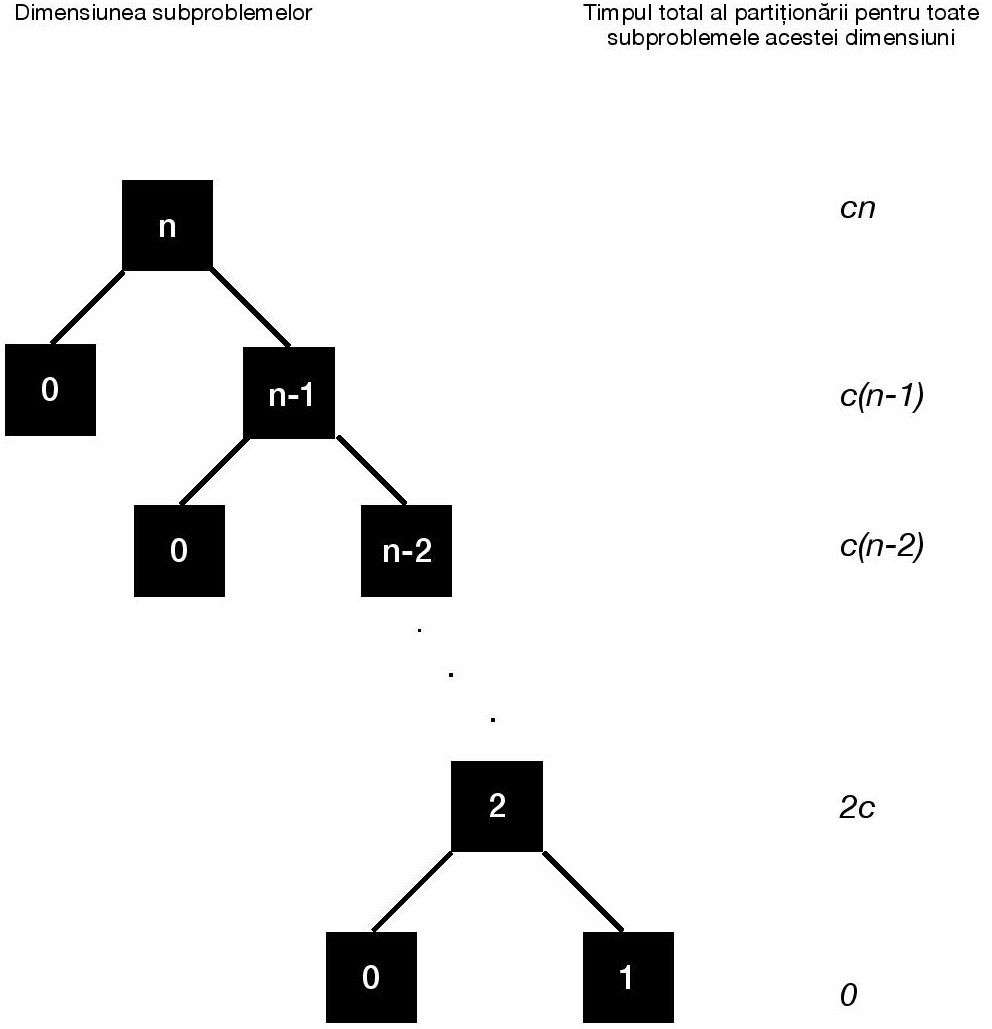
\includegraphics[ width = 12.5 cm]{Worstcase.jpeg}
\end{center}
Când totalizăm timpii de partiționare pentru fiecare nivel, obținem: \\
$ cn + c(n-1) + c(n-2) + ... 2c = c( n + (n-1) + (n-2) + ... 2) = \frac{cn(n-1)}{2} - 1$ \\
  $\implies T(n) = \Theta(n^2)$ \\
   \textbf{Average case: }$T(n) = \Theta(n\log n)$\\
   Dacă toate datele de intrare au probabilități similare, timpul de execuție al cazului mediu este $\Theta(n\log n)$. Intuiția este că dacă inputurile sunt aleatoare, unele partiții vor fi echilibrate și altele nu. Astfel, media partițiilor rezultate va fi un mixt între partiții bune și rele. \\
   \textbf{Best case: $\Theta(n\log n)$ }\\
   Cel mai bun caz posibil apare când partițiile sunt cât mai echilibrate posibil: au dimensiunile egale sau la o diferență de o unitate de celelalte. Cazurile apar când mulțimea are un număr impar de elemente și pivotul este chiar la mijloc după partiție și fiecare partiție are $\frac{(n-1)}{2}$ elemente sau se petrece în momentul în care mulțimea are un număr par de elemente și o partiție are $\frac{(n)}{2}$ și cealaltă are $\frac{(n)}{2} - 1$ elemente. \\
   $T(n) = T(\frac{n}{2}) + T(\frac{n}{2}) + \Theta(n) \implies T(n) = \Theta(n\log n)$
   \item \textbf{Pseudocodul algoritmului}
   \begin{algorithm}
   \caption{: \\ SPRINKLERS-REQUIRED (\emph{left,right, nointervals ,length)}}
    \begin{algorithmic}[1]
        \State $maximum = right[1]$ 
        \State $covered = right[1]$
        \State $count = 1$
        \State $iterator = 2$
        \While {$iterator \leq nointervals$ \textbf{and} $right[iterator] \leq covered$}
            \State $iterator = iterator + 1$
        \EndWhile
         \While {$iterator \leq nointervals$ \textbf{and} $covered \leq length$}
             \While {$left[iterator] \leq covered$ \textbf{and} $iterator \leq nointervals$}
                \If{$right[iterator] > maximum$}
                    \State $maximum = right[iterator]$
                \EndIf
                \State $iterator = iterator + 1$
             \EndWhile
             \If{$maximum \neq covered$}
                    \State $count = count + 1$
             \EndIf
             \State $covered = maximum$
        \EndWhile
        \State \textbf{return } $count$
\end{algorithmic}
\end{algorithm}
\subsubsection{Comparare algoritmi}
   \begin{center}
   \begin{tabular}{|c|c|c|}
        \hline Index algoritm: & $1$ & $2$ \\
        \hline Worst case space complexity: & $\bigcirc(1) $   &$\bigcirc(\log(n)) $\\ 
        \hline Worst case: &$\Theta(n^2)$  &$ \Theta(n^2)$ \\
        \hline Average case: &$ \bigcirc(n^2)$ & $\Theta(n\log n)$\\
        \hline Best case: & $\bigcirc(n)$  & $\Theta(n\log n)$\\
        \hline
   \end{tabular}
   \end{center}
   \textbf{\emph{Observație: }}Al doilea algoritm este mai eficient ca timp de execuție decât primul. Implementarea recursivă a algoritmului de sortare rapidă face ca al doilea algoritm să aibă o complexitate spațială mai mare, comparativ cu primul.
\end{enumerate}
\vspace{10cm}
\section{Date experimentale}
\subsection{Datele de intrare și datele de ieșire}
\begin{enumerate}
  \item Date de intrare:\\
\emph{Linia 1: numărul de aspersoare}\\
\emph{Linia 2: lungimea fâșiei de iarbă}\\
\emph{Linia 3: lățimea fâșiei de iarbă}\\
\emph{Linia 4: poziția primului aspersor}\\
\emph{Linia 5: raza de operare a primului aspersor}\\
.........................................................................................................................\\
\emph{Linia 2*(numărul de aspersoare) + 2: poziția ultimului aspersor}\\
\emph{Linia 2*(numărul de aspersoare) + 3: raza de operare a ultimului aspersor}\\
Caracteristici și proprietăți date intrare:\\
numărul de aspersoare $\in \emph{N}$\\
lungimea, lățimea, pozițiile și razele de acțiune  $\in \emph{R}$\\
    $\forall x \in [\emph{0}, \emph{L}], x \in [a_1, b_1]\bigcup...\bigcup[a_{n},{b_{n}]$, unde: \\
    $a_i = poziția_i - \sqrt{raza_i^2 - (\frac{lățime}{2})^2 } \\
    $b_i = poziția_i + \sqrt{raza_i^2 - (\frac{lățime}{2})^2 }$ \\
    $ 0 \leq a_i \leq b_i \leq lungimea$ și $ 1 \leq i \leq$ număr aspersoare \\
    $0 \leq lățimea \leq lungimea $\\ 
1 $\leq$ numărul de aspersoare\\ 
0 $\leq$ $poziția_i$ $\leq$ lungimea, $\forall$ i $\in$ [1,numărul de aspersoare]
\item Date de ieșire:\\
\emph{Linia 1: numărul minim de aspersoare necesare pentru a uda banda de iarbă}\\
Caracteristici și proprietăți date ieșire:\\
$\forall x \in [\emph{0}, \emph{L}],\exists $i_1 ... i_k$ astfel încât x \in [a_{i_1}, b_{i_1}]\bigcup...\bigcup[a_{i_k},b_{i_k}]$, unde: \\
    $ 1 \leq$ k $\leq$ numărul total de aspersoare, $k \in \emph{N}$, unde k = numărul minim de aspersoare necesare pentru a uda banda de iarbă
\end{enumerate} \\
\subsection{Modalitate de generare}
\\ Pentru numărul maxim al aspersoarelor am definit o constantă, $maxspl$, iar numărul de aspersoare va fi o valoare generată aleator, cuprinsă între $1$ și $maxspl$. Vom memora capetele intervalelor stropite de fiecare aspersor în 2 tablouri unidimensionale, unul pentru capetele din stânga și celălalt, pentru capetele din dreapta. Pentru a asigura corectitudinea datelor de intrare, am generat un număr aleator care reprezintă soluția inițială, unde $1 \leq solinit \leq nosprinklers$. Vom genera $solinit$ intervale, astfel: capătul stâng al primului interval va fi inițializat cu 0, iar pentru capătul drept se va genera o valoare cuprinsă între  $0$ și $maxstep$, o constantă folosită pentru a alege care să fie distanța maximă între capete drepte ale intervalelor inițiale. \\ 
Regula de generare a următoarelor $solinit-1$ intervale este următoarea: capătul stâng al fiecărui interval curent va primi valoare aleatoare cuprinsă între capătul stâng și cel drept al intervalului anterior. Capătul drept al intervalului curent va primi o valoare aleatoare între capătul drept anterior și $maxstep$ + capătul drept al intervalului anterior. Dacă unul dintre capătul drept sau stâng al intervalului actual este egal cu cel anterior, procesul se va repeta.\\
În continuare, lungimea dreptunghiului de iarbă va primi valoarea capătului drept al ultimului interval generat, iar lățimea o valoare cuprinsă între 0 și lungimea fâșiei de iarbă. \\
Pentru a genera celelalte $nosprinklers - solinit$ intervale, vom folosi o variabilă ce primește o valoare aleatoare între 0 și 1. Dacă $solinit$ are valoarea $1$ sau variabila are valoarea $1$, se va apela funcția care inserează un interval inclus într-un alt interval aleator din cele inițiale, în caz contrar, se va apela funcția care inserează un interval nou între 2 intervale inițiale aflate pe poziții consecutive. \\
După ce am generat toate intervalele, vom efectua nosprinklers permutări între pozițiile a 2 intervale selectate random, pentru a face datele de intrare să fie cât mai aleatoare. \\
Vom lista numărul de aspersoare, lungimea și lățimea, fiecare pe o linie. \\
Apoi, pentru fiecare dintre cele nosprinklers aspersoare, vom calcula distanța față de capătul din stânga al liniei care străbate pe orizontală mijlocul fâșiei de iarbă, care este egală cu media aritmetică dintre capătul stâng si cel drept pentru fiecare interval în parte, iar raza se va calcula pe baza ecuației cercului, fiind egală cu $\sqrt{(\frac{lățimea}{2})^2+(capăt dreapta - distanța)^2}.$ \\ De asemenea, valoarea obținută pentru rază se va mări cu valoarea 1,  pentru a se evita cazul în care se aproximează inferior, dacă raza este mai mare decât cea reieșită din ecuația cercului, nu influențează corectitudinea datelor de intrare. Atât distanța, cât și raza obținute pentru fiecare interval în parte se vor printa, fiecare pe o nouă linie. 
\\Așadar, se obțin nosprinklers aspersoare, lungimea și lățimea bandei orizontale de iarbă, precum și distanța față de capătul din stânga al liniei care străbate pe orizontală mijlocul fâșiei de iarbă și raza de operare, pentru fiecare aspersor în parte, cu proprietatea că nu există un punct din banda orizontală de iarbă care să nu fie udat când toate aspersoarele sunt pornite.\vspace{0,5cm}\\
\vspace{0,1cm}
\textbf{\emph{Observație: } } Datele generate de acest algoritm sunt cuprinse între anumite limite.\\
\begin{center}
   \begin{tabular}{|c|c|c|}
        \hline
        \multicolumn{3}{|c|}{\textbf{Limite date de intrare generate:}} \\
        \hline Parametru: & Limită inferioară: & Limită superioară: \\
        \hline Număr aspersoare & \emph{1}   &\emph{maxspl}\\ 
        \hline Lungimea & $0$ &$maxspl*maxstep$\\
        \hline Lățimea &0& $maxspl*maxstep$\\
        \hline Poziția aspersorului &0  &$maxspl*maxstep-\frac{maxstep}{2}$\\
        \hline Rază de acoperire aspersor&1  &$\sqrt{(\frac{maxspl*maxstep}{2})^2 + (\frac{maxstep}{2})^2} + 1$\\
        \hline
   \end{tabular}
   \end{center}
   \vspace{1cm}
\subsection{Pașii și pseudocodul algoritmului de generare al datelor de intrare}
\textbf{\emph{Pasul 1}}: Numărul de aspersoare primește o valoare cuprinsă între 1 și maxspl\\
\textbf{\emph{Pasul 2}}: Se vor genera solinit intervale inițiale, unde solinit este o valoare cuprinsă între 1  și numărul de aspersoare\\
\textbf{\emph{Pasul 3}}: Primul interval generat va avea capătul stâng 0 și cel drept cuprins între 0 și maxstep, unde maxstep este diferența maximă între capătul stâng și drept al unui interval\\ 
\textbf{\emph{Pasul 4}}: Generăm celelalte solnit-1 intervale, după următoarea regulă: capătul stâng al intervalului actual va fi cuprins între capetele intervalului anterior; capătul drept al intervalului actual va fi cuprins între capătul drept al intervalului precedent și capătul drept al intervalului anterior + maxstep\\
\textbf{\emph{Pasul 5}}: Lungimea primește valoarea ultimui capăt dreapta generat\\
\textbf{\emph{Pasul 6}}: Lățimea primește o valoare între 0 și lungime\\
\textbf{\emph{Pasul 7}}: Generăm celelalte nosprinklers-solinit după următoarea regulă: vom genera într-o variabilă valoarea 0 sau 1, dacă valoarea sau solinit au valoarea 1, capetele intervalului generat vor fi cuprinse între capetele unui interval aleator din primele solinit, altfel, capetele intervalului generat vor fi cuprinse între capătul stanga al intervalului poz și capătul dreapta al intervalului poz+1, unde poz este cuprins între 1 și solinit-1. Repetăm procesul până sunt generate toate intervalele.\\
\textbf{\emph{Pasul 8}}: Efectuăm nosprinklers schimbări de indici între 2 intervale random din cele nosprinklers intervale\\
\textbf{\emph{Pasul 9}}: Printăm pe o linie numărul de aspersoare, lungimea și lățimea\\
\textbf{\emph{Pasul 10}}: Înjumătățim lățimea\\
\textbf{\emph{Pasul 11}}: Calculăm poziția și raza fiecărui aspersor și le afișăm pe câte o linie 
\begin{algorithm}
   \caption{: \\RANDOM-DATA-GENERATOR (\emph{maxspl,maxstep)}}
    \begin{algorithmic}[1]
       \State $nosprinklers =$ RANDOM$(1,maxspl)$
\State $solinit =$ RANDOM$(1,nosprinklers)$
\State $left[1] = 0$
\State $right[1] = $RANDOM$(0,maxstep)$
\For{$iterator = 2$ \textbf{to} $solinit$}
    \State $left[iterator] =$ RANDOM$(left[iterator-1],right[iterator-1])$
    \State $right[iterator] =$ RANDOM$(right[iterator-1],right[iterator-1]+maxstep)$
    \If{$left[iterator-1] = left[iterator]$  \textbf{or } $right[iterator-1] = right[iterator]$ }
        \State $iterator = iterator - 1$
    \EndIf
\EndFor
\State $length = right[solinit]$
\State $width = $RANDOM$(0,length)$
\For{$iterator = solinit+1$ \textbf{to} $nosprinklers$}
\State $number1 = $RANDOM$(0,1)$
\If{$number1 = 1$ \textbf{or }$solinit = 1$ }
    \State INSERTION1$(left,right,solinit,iterator)$
\Else{}
    \State INSERTION2$(left,right,solinit,iterator)$
\EndIf
\EndFor
\For{$iterator = 1$ \textbf{to} $nosprinklers$}
\State $number1 = $RANDOM$(1,nosprinklers)$
\State $number2 = $RANDOM$(1,nosprinklers)$
\State $aux=left[number1],left[number1]=left[number2],left[number2]=aux$
\State $aux=right[number1],right[number1]=right[number2],right[number2]=aux$
\EndFor
\State \textbf{print} $nosprinklers, length, width$
\State $width = \frac{width}{2}$
\For{$iterator = 1$ \textbf{to} $nosprinklers$}
\State $distance = \frac{left[iterator]+right[iterator]}{2}$
\State $radius = \sqrt{width^2 +(right[iterator]-distance)^2} + 1$
\State \textbf{print} $distance, radius$
\EndFor
\end{algorithmic}
\end{algorithm}

\section{Proiectarea aplicației}
\subsection{Structura de nivel înalt a aplicației}
\begin{center}
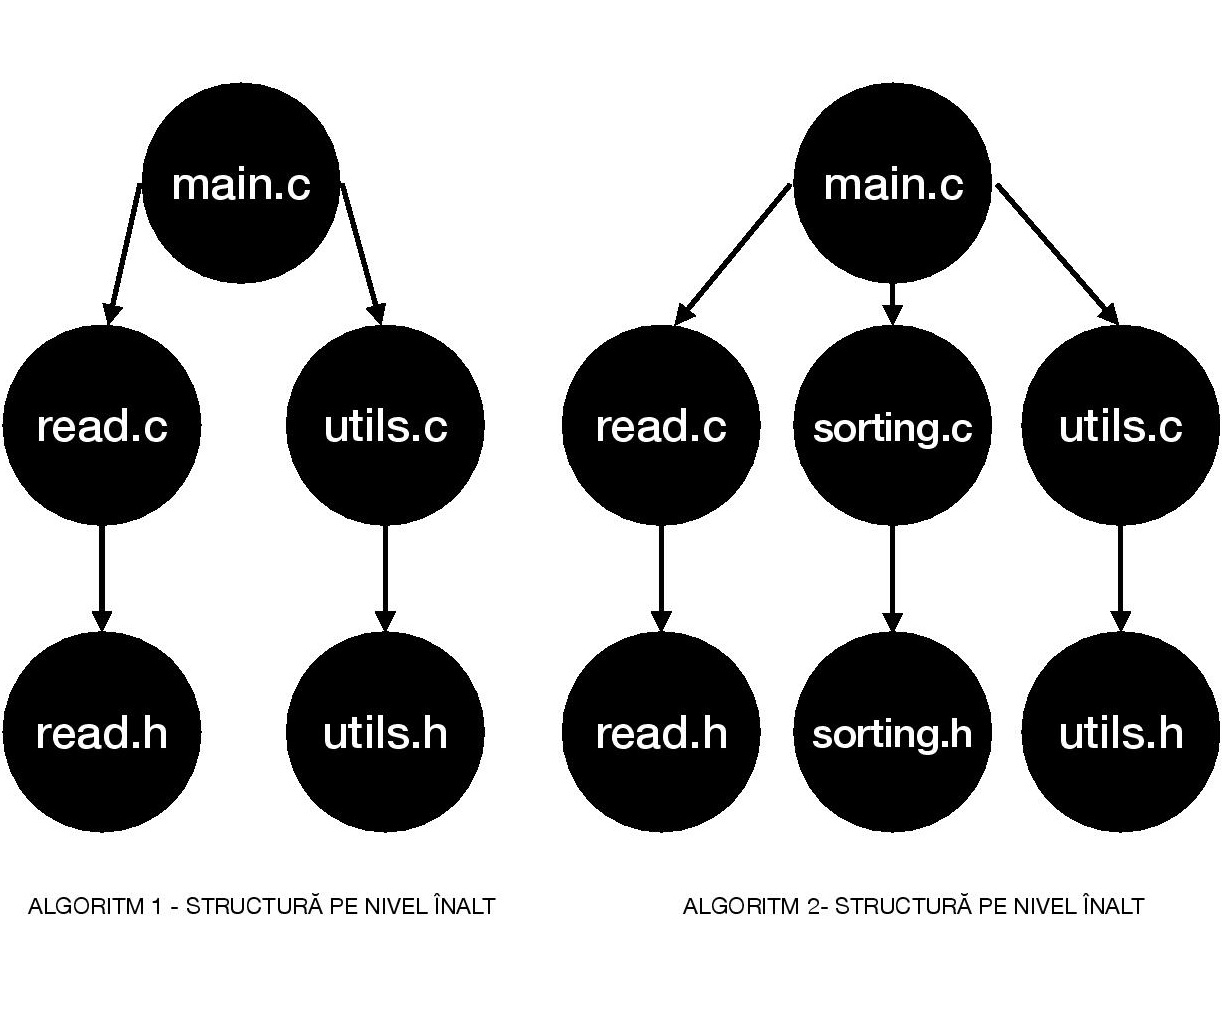
\includegraphics[ width = 15cm]{structuri.jpeg}
\end{center}
\subsection{Datele de intrare }
Sunt cunoscute numărul de aspersoare, lungimea și lățimea benzii orizontale de iarbă, poziția ca distanță față de capătul din stânga al liniei care străbate pe orizontală mijlocul fâșiei de iarbă și raza de acțiune a fiecărui aspersor. \\
Tipul datelor de intrare:
\begin{itemize}
    \item numărul de aspersoare: număr natural $>$ 0( în C unsigned long ) 
    \item lungimea, lățimea și cele \emph{n} distanțe și raze de acțiune ale aspersoarelor sunt numere reale pozitive(float), unde  \emph{n} reprezintă numărul de aspersoare
\end{itemize}
Datele de intrare trebuie să îndeplinească următoarelele proprietăți:
\begin{itemize}
    \item 0 $\leq$ distanța la care este poziționat aspersorul $\leq$ lungimea benzii de iarbă
    \item $\forall x \in [\emph{0}, \emph{L}], x \in [a_1, b_1]\bigcup...\bigcup[a_{n},{b_{n}]$, unde: \\
    $a_i = distanța_i - \sqrt{raza_i^2 - (\frac{lățime}{2})^2 } \\
    $b_i = distanța_i + \sqrt{raza_i^2 - (\frac{lățime}{2})^2 } \\
    $ 0 \leq a_i \leq b_i \leq lungimea$, $ 0 \leq lățimea \leq lungimea $ și $ 1 \leq i \leq n$, unde  \emph{n} reprezintă numărul de aspersoare
\end{itemize}
\subsection{Datele de ieșire }
Se determină și afișează numărul minim de aspersoare necesare pentru a uda fiecare punct din banda de iarbă.\\
Tipul datelor de ieșire:
\begin{itemize}
    \item numărul minim de aspersoare necesare: număr natural(unsigned long), $>$ 0 și $\leq n$ , unde  \emph{n} reprezintă numărul total de aspersoare
\end{itemize}
Datele de ieșire trebuie să îndeplinească următoarelele proprietăți:
\begin{itemize}
    \item $\forall x \in [\emph{0}, \emph{L}],\exists $i_1 ... i_k$, $i_1 \neq i_2 \neq ... \neq i_k $, astfel încât x \in [a_{i_1}, b_{i_1}]\bigcup...\bigcup[a_{i_k},b_{i_k}]$, unde: \\
    $ 1 \leq$ k $\leq$ numărul total de aspersoare, k = numărul minim de aspersoare necesare pentru a uda banda de iarbă 
\end{itemize}
\subsection{Modulele aplicației}
\subsubsection{Algoritm 1:}
\begin{itemize}
    \item \textbf{read}
    \item \textbf{utils}
\end{itemize}
Descriere module:
\begin{enumerate}
    \item \textbf{read}: în acest modul sunt descrise funcții pentru citirea datelor de intrare și formarea corectă a intervalelor care sunt complet acoperite de fiecare aspersor în parte
    \item \textbf{utils}: în acest modul sunt descrise funcții pentru determinarea și returnarea numărului minim de aspersoare care pot uda fiecare punct din banda orizontală de iarbă
\end{enumerate}
\subsubsection{Algoritm 2:}
\begin{itemize}
    \item \textbf{read}
    \item \textbf{utils}
    \item \textbf{sorting}
\end{itemize}
Descriere module:
\begin{enumerate}
    \item \textbf{read}: în acest modul sunt descrise funcții pentru citirea datelor de intrare și formarea corectă a intervalelor care sunt complet acoperite de fiecare aspersor în parte
    \item \textbf{sorting}: în acest modul sunt descrise funcții pentru sortarea crescătoare a intervalelor după capătul stâng și descrescătoare după capătul drept
    \item \textbf{utils}: în acest modul sunt descrise funcții pentru determinarea și returnarea numărului minim de aspersoare care pot uda fiecare punct din banda orizontală de iarbă
\end{enumerate}
\subsection{Procedurile aplicației}
\subsubsection{Algoritm1}
\begin{itemize}
    \item \textbf{read}
    \begin{enumerate}
        \item \textbf{FoundPointX( y, radius )} \\
        Această funcție determină soluția pozitivă din ecuația cercului pentru coordonata carteziană de pe axa Ox. \\\textbf{Parametrii funcției:}
        \begin{description}
        \item[Primul parametru: ]y = număr real ce reprezintă coordonata punctului de pe axa Oy
        \item[Al doilea parametru: ]radius = număr real ce reprezintă raza cercului
        \end{description}
        \\Valorile de retur:\\
        Funcția returnează soluția reală pozitivă de pe axa Ox.
        \item \textbf{ReadingData( left, right, nosprinklers, length, width, available  )}
        \\
        Această funcție citește raza și poziția fiecărui aspersor și formează intervalele din fâșia de iarbă pe care le acoperă complet. \\ \textbf{Parametrii funcției:}
        \begin{description}
        \item[Primul parametru: ]left = o mulțime de valori reale ce reprezintă capătul stâng al tuturor intervalelor din banda de iarbă udate complet de aspersoare
        \item[Al doilea parametru: ]right = o mulțime de valori reale ce reprezintă capătul drept al tuturor intervalelor din banda de iarbă udate complet de aspersoare
        \item[Al treilea parametru: ]nosprinklers = număr natural ce reprezintă numărul de aspersoare 
        \item[Al patrulea parametru: ]length = număr real ce reprezintă lungimea fâșiei de iarbă
        \item[Al cincilea parametru: ]width = număr real ce reprezintă lățimea fâșiei de iarbă
        \item[Al șaselea parametru: ]available = o mulțime de valori naturale ce are valoarea 0 pentru indicele aspersoarelor disponibile pentru testare și o valoare nenulă pentru cele deja testate
        \end{description}
        \\ \textbf{Valorile de retur:}\\
        Funcția este de tip \emph{void} și nu returnează o valoare, este folosită pentru citirea datelor și a atribui valorile corespunzătoare pentru mulțimile left și right.
    \end{enumerate}
    \item \textbf{utils}
    \begin{enumerate}
        \item \textbf{DetermineCurrentBeginning ( left, right, start, end, available)}
        \\
        Această funcție determină aspersorul disponibil cu cu cel mai mic capăt stânga și cel mai mare capăt dreapta dacă sunt mai multe aspersoare cu același capăt stânga. \\ \textbf{Parametrii funcției:}
        \begin{description}
        \item[Primul parametru: ]left = o mulțime de valori reale ce reprezintă capătul stâng al tuturor intervalelor din banda de iarbă acoperite de aspersoare
        \item[Al doilea parametru: ]right = o mulțime de valori reale ce reprezintă capătul drept al tuturor intervalelor din banda de iarbă acoperite de aspersoare
        \item[Al treilea parametru: ]start = număr natural ce reprezintă poziția primului aspersor
        \item[Al patrulea parametru: ]end = număr natural ce reprezintă poziția ultimului aspersor
        \item[Al cincilea parametru: ]available = o mulțime de valori naturale ce are valoarea 0 pentru indicele aspersoarelor disponibile pentru testare și o valoare nenulă pentru cele deja testate
        \end{description}
        \\ \textbf{Valorile de retur:}\\
        Funcția returnează un număr natural care reprezintă indicele aspersorului cu cel mai mic capăt stânga și cel mai mare capăt dreapta dintre cele netestate anterior.
        \item \textbf{MinimumNoSprinklers ( left, right, nosprinklers, available )}
        \\
        Această funcție determină numărul minim de aspersoare ce pot uda complet banda orizontală de iarbă. \\ \textbf{Parametrii funcției:}
        \begin{description}
        \item[Primul parametru: ]left = o mulțime de valori reale ce reprezintă capătul stâng al tuturor intervalelor din banda de iarbă acoperite de aspersoare
        \item[Al doilea parametru: ]right = o mulțime de valori reale ce reprezintă capătul drept al tuturor intervalelor din banda de iarbă acoperite de aspersoare
        \item[Al treilea parametru: ]nosprinklers = număr real ce reprezintă numărul total de aspersoare
        \item[Al patrulea parametru: ]available = o mulțime de valori ce are valoarea 0 pentru indicele aspersoarelor disponibile pentru testare și o valoare nenulă pentru cele deja testate
        \end{description}
        \\ \textbf{Valorile de retur:}\\
        Funcția returnează un număr natural ce reprezintă numărul minim de aspersoare necesare pentru a uda fâșia de iarbă.
    \end{enumerate}
\end{itemize}
\subsubsection{Algoritm2}
\begin{itemize}
    \item \textbf{read}
    \begin{enumerate}
        \item \textbf{FoundPointX( y, radius )} \\
        Această funcție determină soluția reală pozitivă din ecuația cercului pentru coordonata carteziană de pe axa Ox. \\\textbf{Parametrii funcției:}
        \begin{description}
        \item[Primul parametru: ]y = coordonata reală pozitivă a punctului de pe axa Oy
        \item[Al doilea parametru: ]radius = număr real ce reprezintă raza cercului
        \end{description}
        \\Valorile de retur:\\
        Funcția returnează soluția reală pozitivă de pe axa Ox.
        \item \textbf{ReadData( left, right, nosprinklers, length, width )}
        \\
        Această funcție citește raza și poziția fiecărui aspersor și formează intervalele din fâșia de iarbă pe care le acoperă complet. \\ \textbf{Parametrii funcției:}
        \begin{description}
        \item[Primul parametru: ]left = o mulțime de valori reale ce reprezintă capătul stâng al tuturor intervalelor din banda de iarbă acoperite de aspersoare
        \item[Al doilea parametru: ]right = o mulțime de valori reale ce reprezintă capătul drept al tuturor intervalelor din banda de iarbă acoperite de aspersoare
        \item[Al treilea parametru: ]nosprinklers = număr natural ce reprezintă numărul de aspersoare 
        \item[Al patrulea parametru: ]length = număr real ce reprezintă lungimea fâșiei de iarbă
        \item[Al cincilea parametru: ]width = număr real ce reprezintă lățimea fâșiei de iarbă
        \end{description}
        \\ \textbf{Valorile de retur:}\\
        Funcția este de tip \emph{void} și nu returnează o valoare, este folosită pentru citirea datelor și a atribui valorile pentru mulțimile left și right.
         \end{enumerate}
         \item \textbf{sorting}
    \begin{enumerate}
        \item \textbf{Swap(start,end,a,b)} \\
        Această funcție schimbă indicii între 2 aspersoare.\\
        \textbf{Parametrii funcției:}
        \begin{description}
        \item[Primul parametru: ]left = o mulțime de valori reale ce reprezintă capătul stâng al tuturor intervalelor din banda de iarbă acoperite de aspersoare
        \item[Al doilea parametru: ]right = o mulțime de valori reale ce reprezintă capătul drept al tuturor intervalelor din banda de iarbă acoperite de aspersoare
        \item[Al treilea parametru: ]a = număr natural ce reprezintă indicele primului aspersor 
        \item[Al patrulea parametru: ]b = număr natural ce reprezintă indicele celui de-al doilea aspersor
        \end{description}
        \\\textbf{Valorile de retur:}\\
        Funcția este de tip \emph{void} și nu returnează o valoare, dar realizează schimbarea de indici între aspersoare.
        \item \textbf{Partition(left, right, low, high)}
        \\
         Această funcție ia ultimul element ca pivot, și determină poziția corectă a pivotului(aspersorului), plasând toate aspersoarele mai mici în stânga pivotului și cele mai mari în dreapta. \\ \textbf{Parametrii funcției:}
        \begin{description}
        \item[Primul parametru: ]left = o mulțime de valori reale ce reprezintă capătul stâng al tuturor intervalelor din banda de iarbă acoperite de aspersoare
        \item[Al doilea parametru: ]right = o mulțime de valori reale ce reprezintă capătul drept al tuturor intervalelor din banda de iarbă acoperite de aspersoare
        \item[Al treilea parametru: ]low = număr natural ce reprezintă cel mai mic indice
        \item[Al patrulea parametru: ] high = număr natural ce reprezintă cel mai mare indice 
        \end{description}
        \\ \textbf{Valorile de retur:}\\
        Funcția returnează un număr natural ce reprezintă poziția pivotului selectat în cadrul mulțimii.
        \item \textbf{QuickSort(left, right, low, high)} \\
        Această funcție sortează crescător aspersoarele după capătul din stânga și descrescător după cel din dreapta. \\
        \textbf{Parametrii funcției:}
        \begin{description}
         \item[Primul parametru: ]left = o mulțime de valori reale ce reprezintă capătul stâng al tuturor intervalelor din banda de iarbă acoperite de aspersoare
        \item[Al doilea parametru: ]right = o mulțime de valori reale ce reprezintă capătul drept al tuturor intervalelor din banda de iarbă acoperite de aspersoare
        \item[Al treilea parametru: ]low = număr natural ce reprezintă cel mai mic indice
        \item[Al patrulea parametru: ] high = număr natural ce reprezintă cel mai mare indice
        \end{description}
        \\ \textbf{Valorile de retur:}\\
        Funcția este de tip \emph{void} recursivă și nu returnează o valoare, în schimb se auto-apelează până când se realizează sortarea aspersoarelor.
    \end{enumerate}
        \item \textbf{utils}
    \begin{enumerate}
        \item \textbf{SprinklersRequired( left, right, nosprinklers, length )} \\
        Această funcție determină numărul minim de aspersoare necesare pentru a uda fâșia de iarbă. \\
        \textbf{Parametrii funcției:}
        \begin{description}
         \item[Primul parametru: ]left = o mulțime de valori reale ce reprezintă capătul stâng al tuturor intervalelor din banda de iarbă acoperite de aspersoare
        \item[Al doilea parametru: ]right = o mulțime de valori reale ce reprezintă capătul drept al tuturor intervalelor din banda de iarbă acoperite de aspersoare
        \item[Al treilea parametru: ]nosprinklers = număr natural ce reprezintă numărul de aspersoare 
        \item[Al patrulea parametru: ]length = număr real ce reprezintă lungimea fâșiei de iarbă
        \end{description}
        \\ \textbf{Valorile de retur:}\\
        Funcția returnează un număr natural ce reprezintă numărul minim de aspersoare necesare pentru a uda fâșia de iarbă.
    \end{enumerate}
\end{itemize}
\vspace{10cm}
\section{Rezultate și concluzii}
\subsection{Rezultate}
Am colectat datele de ieșire și media timpului de execuție al celor 2 algoritmi,atât în C, cât și în Python, pentru date de intrare de dimensiuni din ce în ce mai mari. Rezultatele obținute pot fi vizualizate aici:
   \begin{center}
   \begin{tabular}{|c|c|c|c|c|c|c|c|c|c|c|}
       \hline
        Nr. aspersoare: &1000 &1500 &2500 &5000 &10000 &15000 &25000 &50000 &75000 &100000\\ \hline
       Date ieșire Alg. 1C: &122 &210 &226 &130 &394 &781 &5260 &4907 &2571 &1401\\
        \hline
       Date ieșire Alg. 1Py: &122 &210 &226 &130 &394 &781 &5260 &4907 &2571 &1401\\ 
        \hline
        Date ieșire Alg. 2C: &122 &210 &226 &130 &394 &781 &5260 &4907 &2571 &1401\\ 
        \hline
       Date ieșire Alg. 2Py: &122 &210 &226 &130 &394 &781 &5260 &4907 &2571 &1401\\ 
        \hline
         T. Execuție Alg. 1C: &$0,0001$ &$0,009$ &$0,031$ &$0,032$ &$0,124$ &$0,359$ &$3,61$ &$5,33$ &$4,14$ &$3,39$\\
        \hline
         T. Execuție Alg. 1Py: &$0,071$ &$0,1375$ &$0,2815$ &$0,43$ &$1,48$ &$3,7$ &$39,47$ &$75,53$ &$60,08$ &$43,17$\\ 
        \hline
         T. Execuție Alg. 2C: &$0,0009$ &$0,001$ &$0,015$ &$0,015$ &$0,046$ &$0,047$ &$0,093$ &$0,167$ &$0,203$ &$0,265$\\ 
        \hline
        T. Execuție Alg. 2Py: &$0,007$ &$0,019$ &$0,03$ &$0,162$ &$0,131$ &$0,174$ &$0,259$ &$0,566$ &$0,65$ &$0,78$\\
        \hline
   \end{tabular}
   \end{center}
   Pentru a înțelege semnificația datelor din tabelul de mai sus, am creat o serie de diagrame, pentru a observa comportamentul fiecărui algoritm și a-i compara.
   \subsubsection{Evoluția fiecărui algoritm}
   \begin{center}
    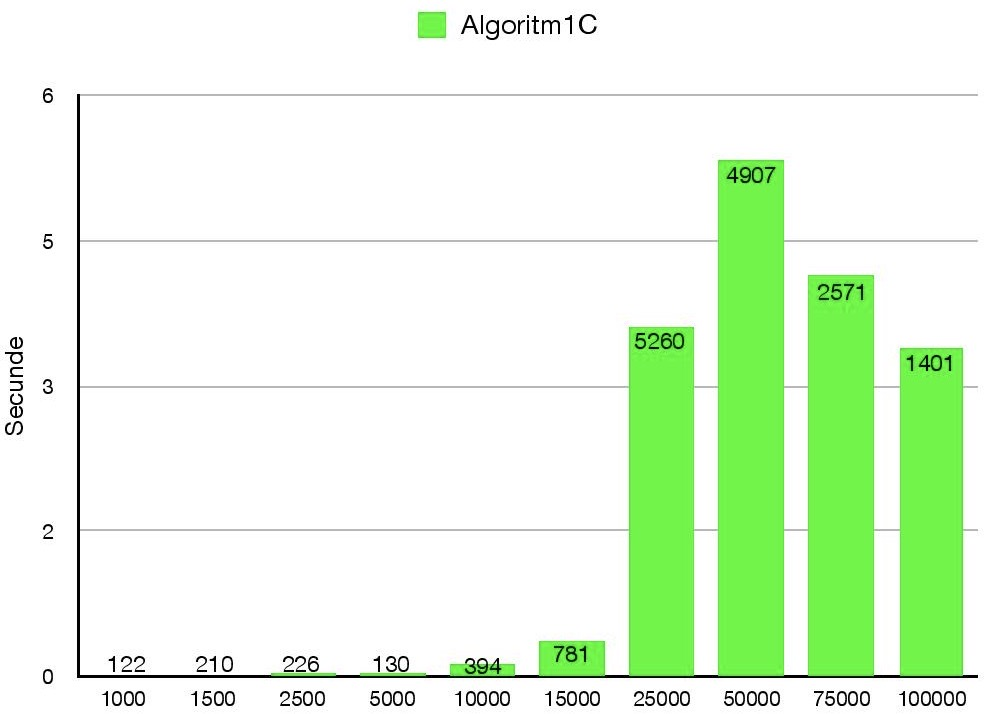
\includegraphics[width = 14cm]{alg1C.jpeg}  
   \end{center}
    \begin{center}
     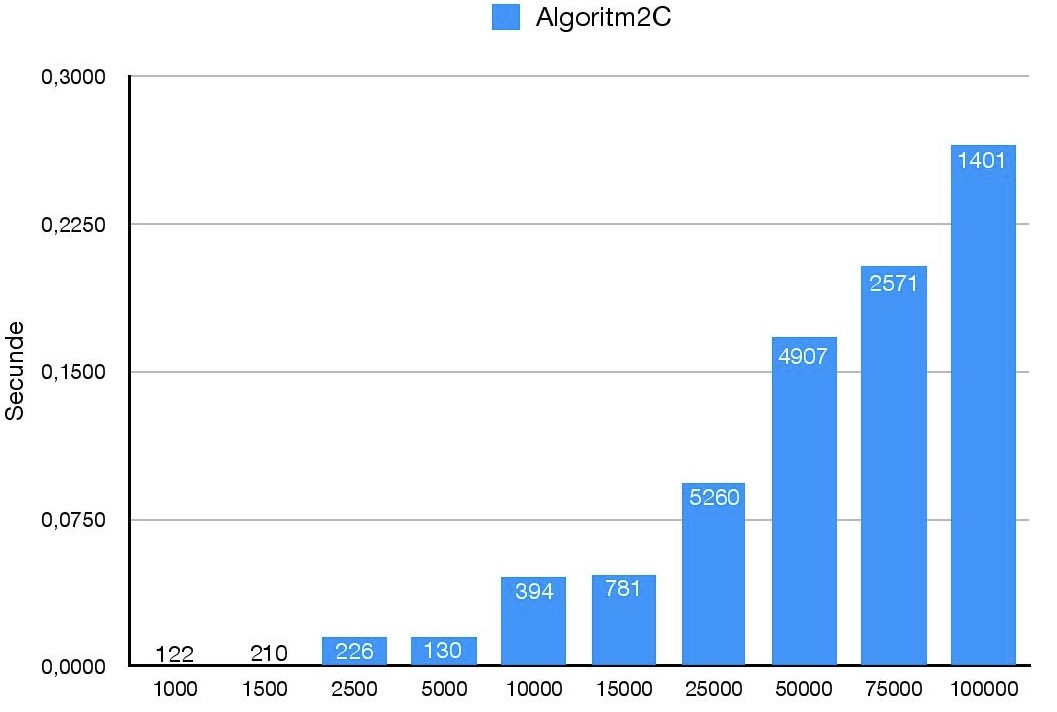
\includegraphics[width = 15cm]{alg2C.jpeg}   
    \end{center}
    \begin{center}
     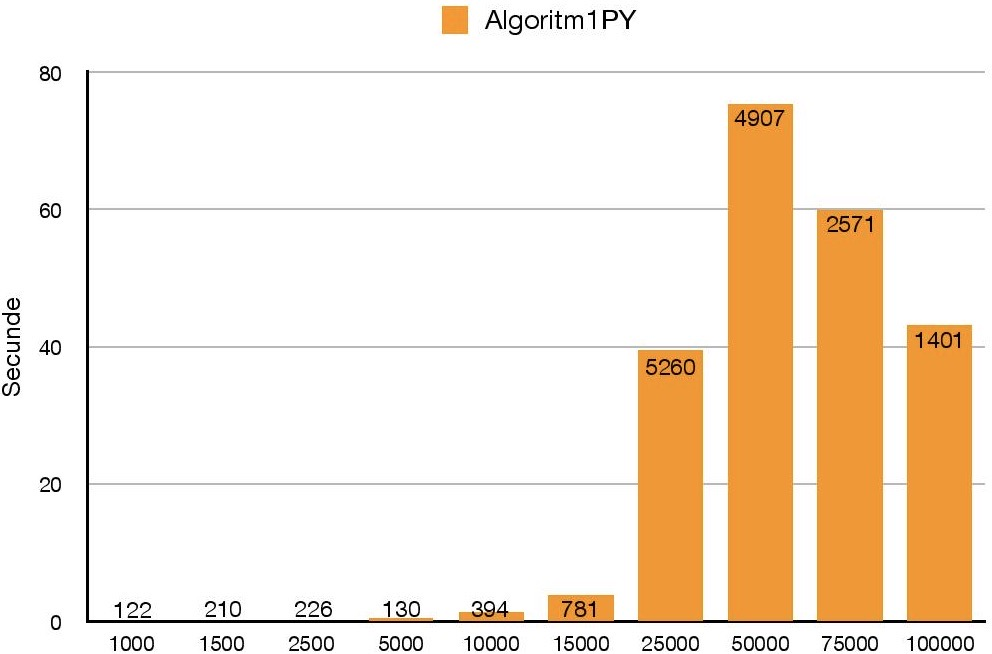
\includegraphics[width = 14cm]{alg1PY.jpeg}   
    \end{center}
   \begin{center}
    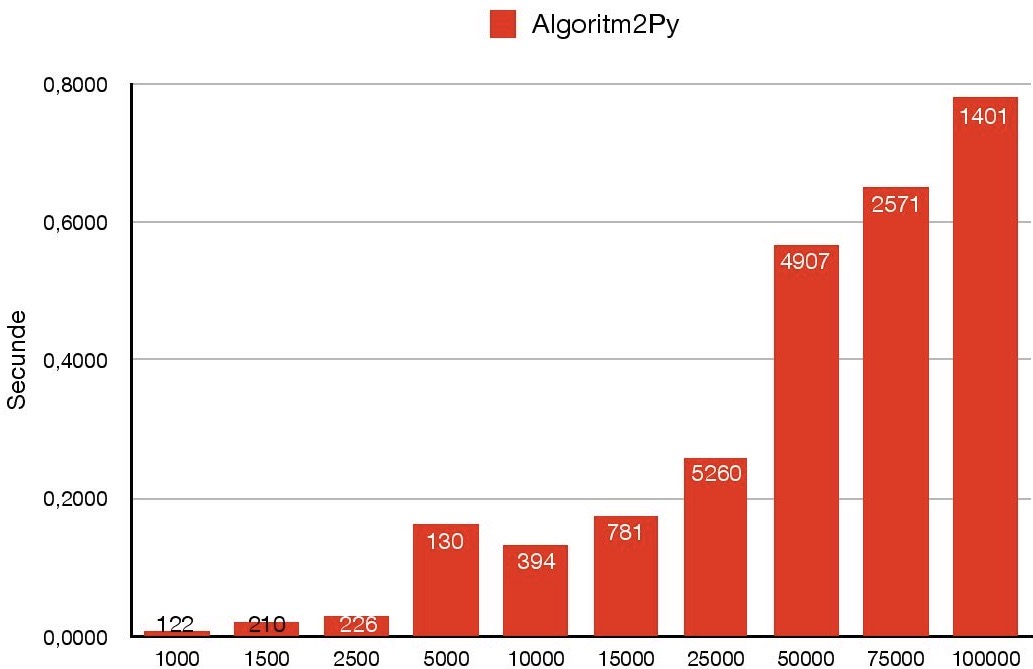
\includegraphics[width = 15cm]{alg2PY.jpeg}  
   \end{center}
   \vspace{1cm}
   \textbf{\emph{Observații: } } 
   \item Timpul de execuție al primului algoritm este influențat într-un procentaj mai mare de numărul de aspersoare selectate pentru fiecare intrare de date decât de dimensiunea lor, deoarece pentru fiecare aspersor nou selectat se parcurge de încă 2 ori mulțimea tuturor aspersoarelor. 
   \item Timpul de execuție al celui de-al doilea algoritm este influențat, predominant, de dimensiunea datelor de intrare, deoarece acestea trebuie sortate și ulterior parcurse liniar.
   \item În cazul ambilor algoritmi, evoluția timpului de execuție între implementarea în C și cea în Python este simetrică.
   \item Toți algoritmii oferă aceleași date de ieșire, ci anume, numărul de aspersoare minime. \\
   Pentru a verifica dacă datele de ieșire sunt corecte, am testat implementările pentru date de intrare cu un număr redus de aspersoare(10-100), care să acopere toate cazurile și să îmi permită să aflu cu ușurință soluția  corectă. Am comparat intervalele calculate de aplicație și cele calculate de mine, precum și răspunsurile. Numărul minim de aspersoare corect și cel returnat de algoritm au fost mereu identice. Am remarcat, însă, că deși intervalele se formează cu formule identice în C și Python, acestea sunt similare, dar nu mereu egale, din cauza aproximărilor diferite din cele 2 limbaje de programare, existând posibilitatea unor rezultate diferite afișate în Python față de C, în cazuri excepționale, numerele minime de aspersoare determinate fiind apropiate, dar nu identice.
   \subsubsection{Comparare performanțe algoritmi}
    \begin{center}
    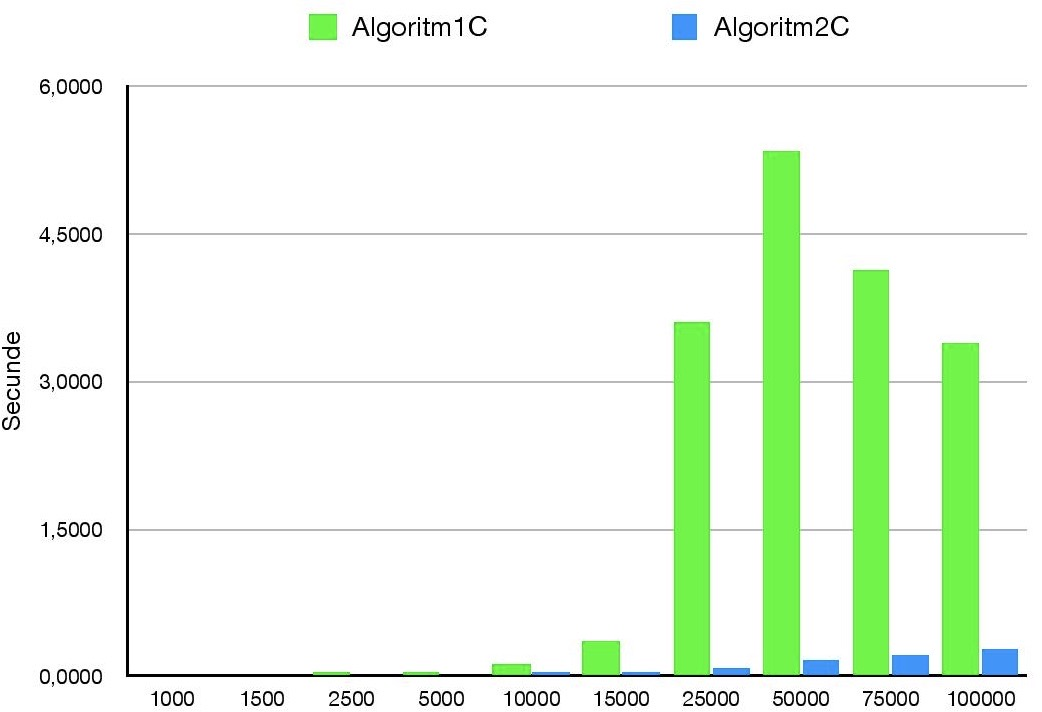
\includegraphics[width = 12cm]{alg1Cvsalg2C.jpeg}  
   \end{center}
    \begin{center}
    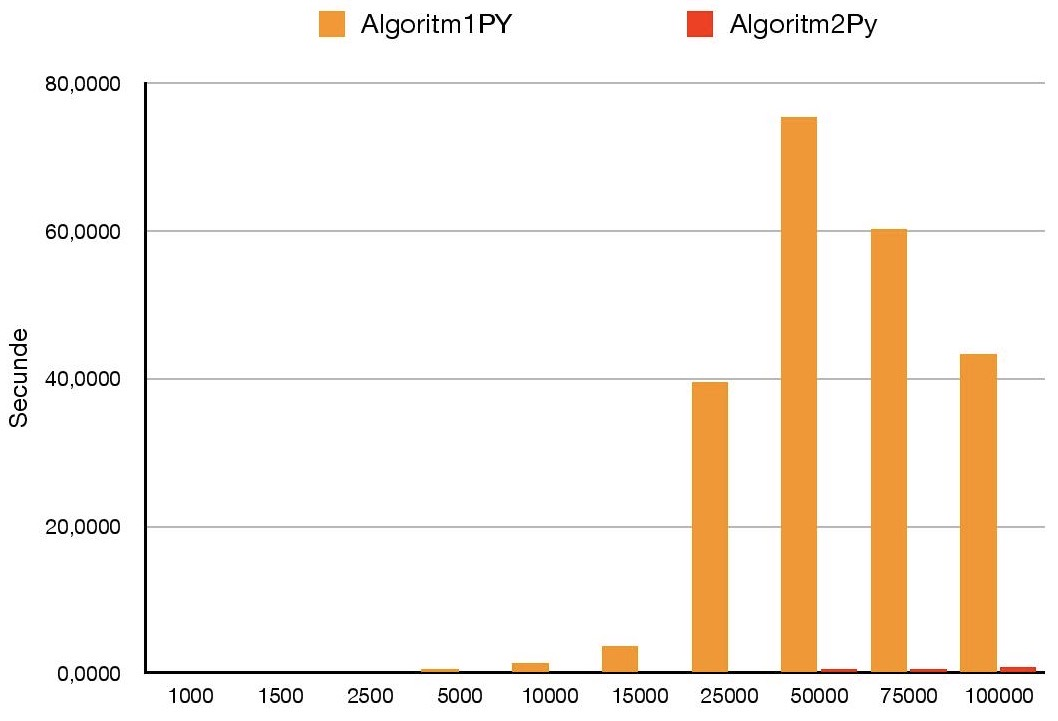
\includegraphics[width = 12cm]{alg1PYvsalg2Py.jpeg}  
   \end{center}
   \textbf{\emph{Observații: } } 
   \item Cel de-al doilea algoritm oferă performanțe mai mult mai bune, atât în C, cât și în Python. De exemplu, în cazul celor 50000 date de intrare, În limbajul C este aproximativ 32 de ori mai rapid, iar în limbajul Python, de 133 de ori mai rapid decât primul algoritm. 
   \subsubsection{Comparare implementări C și Python}
    \begin{center}
    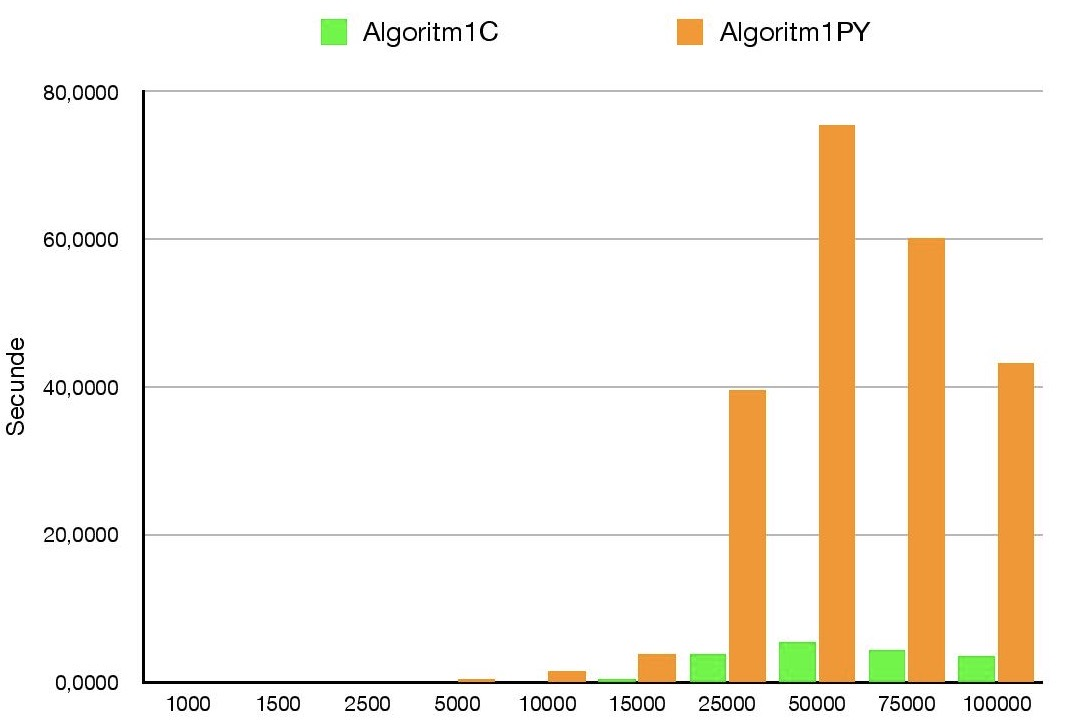
\includegraphics[width = 12cm]{alg1CvsPY.jpeg}  
   \end{center}
    \begin{center}
    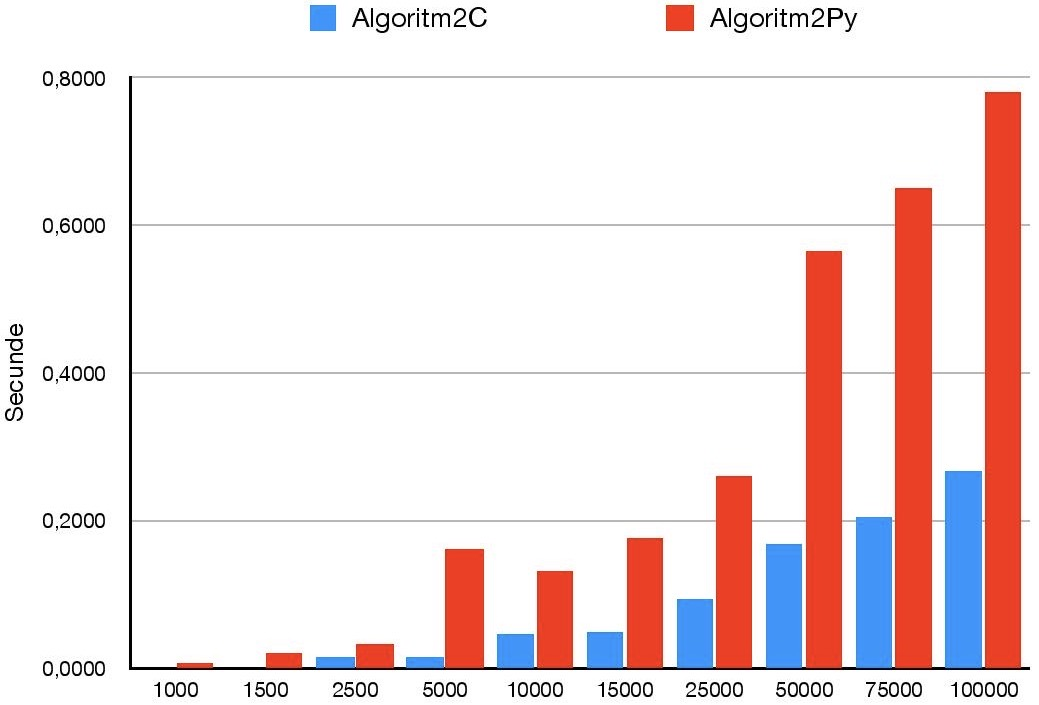
\includegraphics[width = 12cm]{alg2CvsPY.jpeg}  
   \end{center}
   \textbf{\emph{Observații: } } 
   \item Implementările din limbajul C sunt mai rapide decât cele din Python. Acest fapt se datorează diferențelor dintre limbaje: Python este un limbaj interpretat, C este compilat, Python nu are primitive, toate fiind obiecte,listele Python pot conține obiecte de diferite tipuri, etc. 
   \subsubsection{Comparare toate implementările}
     \vspace{1cm}
     \begin{center}
      \includegraphics[width = 14cm]{AnalizăDeTimp.jpeg}  
     \end{center}
\subsection{Concluzii}
Am reușit implementarea a 2 algoritmi diferiți pentru determinarea numărului minim de aspersoare necesare pentru a uda o banda orizontală de iarbă, de dimensiune \emph{L*l}, dacă acestea sunt poziționate centrat vertical pe linia orizontală ce străbate mijlocul fâșiei de iarbă. \\
A fost o experiență interesantă și foarte utilă, deoarece mi-am dezvoltat abilitățile de programare în limbajul C și am învățat o mulțime de lucruri noi: să îmi generez singur date de intrare valide pentru programe, să concep și să implementez algoritmi, să analizez complexitatea algoritmilor, precum și limbajele de programare \LaTeX~\ și Python, cu care nu am mai avut tangențe până la această temă de casă.\\
Evident, a fost o adevărată provocare ca în decurs de câteva zile, să învăț 2 limbaje complet necunoscute, dar acest proiect mi-a arătat ușurința cu care se poate învăța un limbaj de programare dacă deja știi cel puțin încă unul.  
\\Pe viitor, plănuiesc să îmi dezvolt abilitățile în limbajele de programare în C și Python, dar și să îmi lărgesc orizonturile, învățând și alte limbaje de programare, precum: Java și PHP.
\vspace{15cm}

\begin{thebibliography}{9}
	\bibitem{cormen09}
	  Thomas H. Cormen and Charles E. Leiserson and Ronald L. Rivest and Clifford Stein,
	  \emph{Introduction to Algorithms}.
	  MIT Press,
	  3rd Edition,
	  2009.

    \bibitem{wikipedia}
     wikipedia,\url{https://en.wikipedia.org/wiki/Wikipedia:LaTeX_symbols},
     accessed in April 2020.

    \bibitem{geeksforgeeks}
     geeksforgeeks,\url{https://www.geeksforgeeks.org/quick-sort/},
     accessed in April 2020.
     
     \bibitem{python}
     python, \url{https://docs.python.org/3/library/functions.html},
     accessed in April 2020.
     
     \bibitem{w3schools}
     w3schools, \url{https://www.w3schools.com/python/default.asp},
     accessed in April 2020.
    
     \bibitem{hackerearth}
     hackerearth,\url{https://www.hackerearth.com/practice/algorithms/greedy/basics-of-greedy-algorithms/tutorial/},
     accessed in April 2020.
    
     \bibitem{kahnacademy}
     kahnacademy,\url{https://www.khanacademy.org/computing/computer-science/algorithms/quick-sort/a/analysis-of-quicksort},
     accessed in May 2020.
\end{thebibliography}
\end{document}
